
\documentclass[aps, prd, superscriptaddress,twocolumn,amsmath,amssymb,nofootinbib]{revtex4-1}
%\documentclass[prl,superscriptaddress,amsmath]{revtex4-1}
\usepackage{graphicx}
%\usepackage{float}
\usepackage{color}
%\usepackage{tensor}
\usepackage{epstopdf,cancel,ulem}
\usepackage{epsf,latexsym,bbm,euscript}
\usepackage{amssymb,amsmath}
\usepackage{mathtools} %used in this file for the command \coloneqq -> :=
\usepackage{times,graphics}
%\usepackage{subfig}
\usepackage{soul,xcolor}
\usepackage{epsfig}
%\usepackage{geometry}

\linespread{1.0}
% \usepackage{geometry}
\usepackage{graphicx}
%\usepackage{maplestd2e}
%\usepackage[dvipsnames]{xcolor}
%\usepackage{epstopdf}
%\usepackage[abs]{overpic}
%\usepackage{color}
%\usepackage{comment}
%\usepackage{float}
% \usepackage{showkeys}
%\usepackage{booktabs}
\usepackage[colorlinks]{hyperref}
\usepackage{nicefrac}


%%%%%%%%%%%%%%%%%%%%%%%%%%%%%%%%%%%%%%%%%%%%%%%%%%%%%%
%% definitions
\newcommand{\ph}{\varphi}
\newcommand{\tht}{\vartheta}
\newcommand{\eps}{\varepsilon}
\newcommand{\one}{\textsc{i}}

 \newcommand{\dm}{n}

\newcommand{\tens}[1]{{\boldsymbol{#1}}} 
\newcommand{\pa}{{\tens{\partial}}}

\newcommand{\be}{\begin{equation}}
\newcommand{\ee}{\end{equation}}
\newcommand{\ba}{\begin{eqnarray}}
\newcommand{\ea}{\end{eqnarray}}

\newcommand{\beq}{\begin{equation}}
\newcommand{\eeq}{\end{equation}}
\newcommand{\beqa}{\begin{eqnarray}}
\newcommand{\eeqa}{\end{eqnarray}}
\newcommand{\nn}{\nonumber}
\newcommand{\tcb}{\textcolor{blue}}
\newcommand{\tcr}{\textcolor{red}}


\newcommand{\hook}{\raisebox{-0.35ex}{\makebox[0.6em][r]
{\scriptsize $-$}}\hspace{-0.15em}\raisebox{0.25ex}{\makebox[0.4em][l]{\tiny
 $|$}}}
\newcommand{\cwedge}[1]{\mathop{\wedge}_{{}^{#1}} }

\newcommand{\even}{{\mathrm{e}}}
\newcommand{\odd}{{\mathrm{o}}}
\newcommand{\KY}{{\scriptscriptstyle\mathrm{KY}}}
\newcommand{\SN}{{\scriptscriptstyle\mathrm{SN}}}

\newcommand{\fiber}{\boldsymbol}

\newcommand{\lied}{\mathcal{L}}
%\newcommand{\cd}[1]{\frac{\partial}{\partial{#1}}}
\newcommand{\cd}[1]{\frac{\eth}{\partial{#1}}}
\newcommand{\cv}[1]{{\partial}_{#1}}

\newcommand{\Ric}{{\mathrm{Ric}}}
\newcommand{\curvop}{{\boldsymbol{\mathsf{R}}}}
\newcommand{\sccur}{{\mathcal{R}}}
\newcommand{\detg}{{\mathfrak{g}}}


\newcommand{\gc}[2]{{[\mspace{-4mu}\lvert#1,#2\rvert\mspace{-4mu}]}}
\newcommand{\bgc}[2]{{\bigl[\mspace{-4.4mu}\lvert#1,#2\rvert\mspace{-4.4mu}\bigr]}}
\newcommand{\Bgc}[2]{{\biggl[\mspace{-5mu}\Bigl\lvert#1,#2\Bigr\rvert\mspace{-5mu}\biggr]}}

\newcommand{\lst}[1]{\langle{#1}\rangle}


\newcommand{\ef}{E}
\newcommand{\efr}{{\underset{\raisebox{0.5ex}{$\scriptscriptstyle\rightarrow$}}{e}\mspace{-2mu}}}
\newcommand{\Xfr}{{\overset{\raisebox{-0.5ex}{$\scriptscriptstyle\rightarrow$}}{X}\mspace{-1mu}}}



\newcommand{\spcm}{{\mspace{14.5mu}}}                  % space with width of minus
\newcommand{\nquad}{{\mspace{-20mu}}}                  % negative quad
\newcommand{\textdash}{{\text{-}}}                     % text dash for equations



\newcommand{\KV}[1]{\xi_{(#1)}}
\newcommand{\KT}[1]{K_{(#1)}}
\newcommand{\PKV}{\xi}
\newcommand{\CCKY}[1]{h^{(#1)}}


\newcommand{\A}[1]{A^{\!(#1)}}
\newcommand{\B}[1]{B^{\!(#1)}}
\newcommand{\Bo}[1]{\mathcal{B}^{(#1)}}
\newcommand{\Vo}{\mathcal{V}}
\newcommand{\C}[1]{{\cal{#1}}}
\newcommand{\psc}[1]{\Psi_{#1}}
\newcommand{\chc}[1]{\mathcal{X}_{#1}}
\newcommand{\psf}[1]{\tilde\Psi_{#1}}
\newcommand{\chf}[1]{\tilde{\mathcal{X}}_{#1}}

\newcommand{\clfm}[1]{{\slash\mspace{-9.5mu}{#1}}}
\newcommand{\Ha}{{\cal{H}}}


\def\Gdp{\Gamma_{\mathrm{DP}}}
\def\Gktm{\Gamma_{\mathrm{KTM}}}
\def\tGktm{\tilde{\Gamma}_{\mathrm{KTM}}}

%\newcommand{\comment}[2][]{\noindent\hspace{-4em}\framebox{\parbox{6.5in}{\textsf{\small\emph{Comment by #1:} #2}}}\medskip}

%\input{tex_defs}

%%%%%%%%%%%%%%%%%%%%%%%%%%%%%%%%%
%%% definitions of common symbols %%%%%%%
% two particle density operator \
\def\Rt{{\rho}_{12}(t)}
% one particle density operator 
\def\rt{{\rho}(t)}
\def\drho{\dot\rho}
% bra and  kets
\newcommand{\ket}[1]{\lvert \, #1\rangle}
\newcommand{\bra}[1]{\langle #1 \, \rvert}
\newcommand{\braket}[2]{\langle #1 \, | \, #2 \rangle}
\newcommand{\mean}[1]{\langle #1 \rangle}
% "hats"
\newcommand{\h}[1]{\hat#1{}}
%trace 
\def\Tr{{\textrm{Tr}}}


\newcommand{\Radd}[1]{\textcolor{blue}{#1} }
\newcommand{\Rcomm}[1]{\textcolor{blue}{\bf{[#1]}} }
\newcommand{\Nadd}[1]{\textcolor{violet}{#1} }
\newcommand{\Ncomm}[1]{\textcolor{violet}{\bf{[#1]}} }
\newcommand{\f}{\textcolor{cyan}}
\newcommand{\green}{\textcolor{green}}
\newcommand{\mz}[1]{\textcolor{cyan}{#1} }
\newcommand{\mzc}[1]{\textcolor{cyan}{\bf{[#1]}} }
\newcommand{\red}[1]{\textcolor{red}{#1}}

\begin{document}
\begin{titlepage}
    \begin{center}
        \vspace*{3cm}
        
       \textbf{\huge Using Decoherence Rate Minimization to Test the KTM Model's Global Case}
               
        \vspace{1.5cm}
        \textbf{Jamie Breault}
        
        \today
        
        \vspace{1.5cm}
        A report presented as partial fulfilment of the\\
        requirements of Physics 437B 
        \vspace{3cm}
        \end{center}
        
        Many models have been proposed to describe gravity according to the principles of quantum mechanics. However, until direct experimental evidence of quantum gravity is found, gravity being fundamentally classical remains a valid possibility. Kafri, Taylor, and Milburn have purposed two models of classical gravity, the pairwise case and the global case. Altamirano, Corona-Ugalde, Mann, and Zych have compared the pairwise maximum theoretical visibility estimate to the results of atomic fountain interference experiments using decoherence rate minimization. Here, I follow a similar process to obtain the maximum theoretical visibility estimate for the global case instead, and I show that this estimate is inconsistent with values determined experimentally.
    
    \newpage
\end{titlepage}
\onecolumngrid
\pagenumbering{roman}
\tableofcontents
\makeatletter
\let\toc@pre\relax
\let\toc@post\relax
\makeatother
\newpage
\listoffigures
\newpage
\onecolumngrid
%\raggedright
\section{Introduction}
\pagenumbering{arabic}
Presently, one of the greatest problems in theoretical physics is unifying Einstein's theory of general relativity, which describes gravity, with quantum mechanics, which describes the other three fundamental forces. Many models have been proposed to describe gravity according to the principles of quantum mechanics, including loop quantum gravity and string theory \cite{PI}. However, there is not yet any direct observational evidence of quantum gravity \cite{no_QG_evidence}, thus gravity being fundamentally classical remains a valid possibility.

Measurement-feedback models of gravity purposed by Kafri, Taylor, and Milburn (KTM) \cite{KTM1, KTM2, KTM3} describe a mechanism by which gravity could be a classical channel, where classicality is defined as the inability to increase the entanglement of a system. Measurement-feedback models of gravity require agents to conduct weak measurements of particles' positions and then give corresponding feedback to the other particles in the system \cite{P6}. These agents are referred to as ancillae \cite{P2}. Under the KTM model's pairwise case, a system requires two ancillae for each pair particles present \cite{P3}, whereas only one ancillae is required for each particle in the global case.

Atomic fountain interference experiments such as those done by Kovachy et al. \cite{kovachy} can be used to test the validity of global gravity. To do so, the maximum visibility predicted by the model must be derived and compared to experiment. There are two methods that can be used to estimate maximum visibility, one involves decoherence rate minimization and the other involves heating rate minimization \cite{P3}. The maximum visibility estimates produced by these methods may not be equal. The true theoretical maximum visibility is the greater of the two estimates. With both pairwise visibility estimates being known, determined by Altamirano et al. and Breault \cite{P3, breault}, the next step is to determine the global visibility estimates. Here, I determine the DRM maximum visibility estimate for the global case and I compare the estimate to the values determined experimentally.

%%%%%%%%%%%%%%%%%%%%%%%%%%%%%%%%%%%%%%%%%%%%%%%%%%%%%

\section{The KTM Model}

All four fundamental forces are either a quantum or classical channel (fig~\ref{Channels}), the difference being that quantum channels can increase the entanglement of a system and classical channels can not. To illustrate the process by which electromagnetism, a quantum channel, increases entanglement, consider a simple system of two electrons. Let one electron be in a spacial superposition, thus producing a quantum electrical potential. The other electron, being present in the quantum potential, is forced into a state of superposition as well due to the potential's quantum nature. The quantum potential entangles the two electrons. If an observation is made on either of the electrons, both electrons undergo decoherence because of their entanglement. Decoherence is the process of superposition size decreasing due to observation \cite{P6}.

 \begin{figure*}[ht!]
 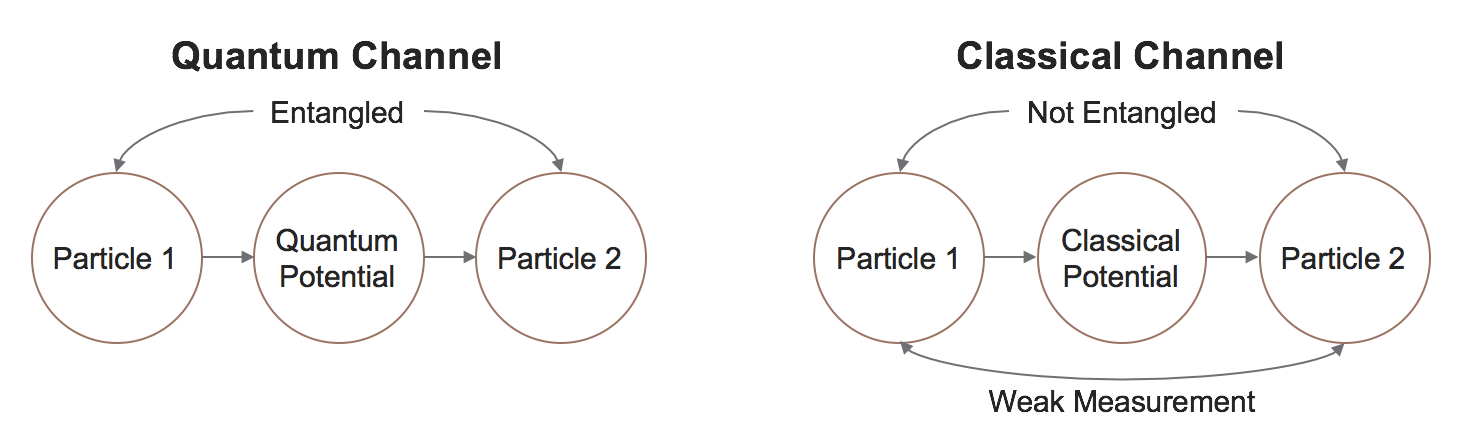
\includegraphics[width=0.8\textwidth]{Channel.png} 
\caption{Diagrams highlighting the differences between quantum channels (left) and classical channels (right).}
\label{Channels}
\end{figure*}

An example of a classical channel is gravity under the KTM model. In this model, gravity is propagated by force carrying particles called ancillae using a measurement-feedback mechanism. To illustrate this mechanism, consider a simple system of two gravitationally interacting particles (fig.~\ref{measurement-feedback}). Each particle interacts with an ancilla, and these initial interactions are referred to as measurements because the ancillae are conducting weak measurements of the particles' positions. Each ancilla then interacts with the other particle, giving the particles feedback that depends on the outcome of the earlier measurement. The position of each particle then shifts as a result of the feedback. These interactions occur continually, over infinitesimal time scales \cite{P2}. These measurement and feedback interactions are equivalent to the particles conducting classical estimates of the surrounding potential. The pair of particles therefore never become entangled \cite{P6}. Note, if gravity is a classical channel, that does not imply that the entanglement of a gravitationally interacting system of particles can not increase, it only implies that the entanglement can not increase due to gravity. Entanglement can still increase through any quantum channel the particles can interact through.

 \begin{figure*}[ht!]
 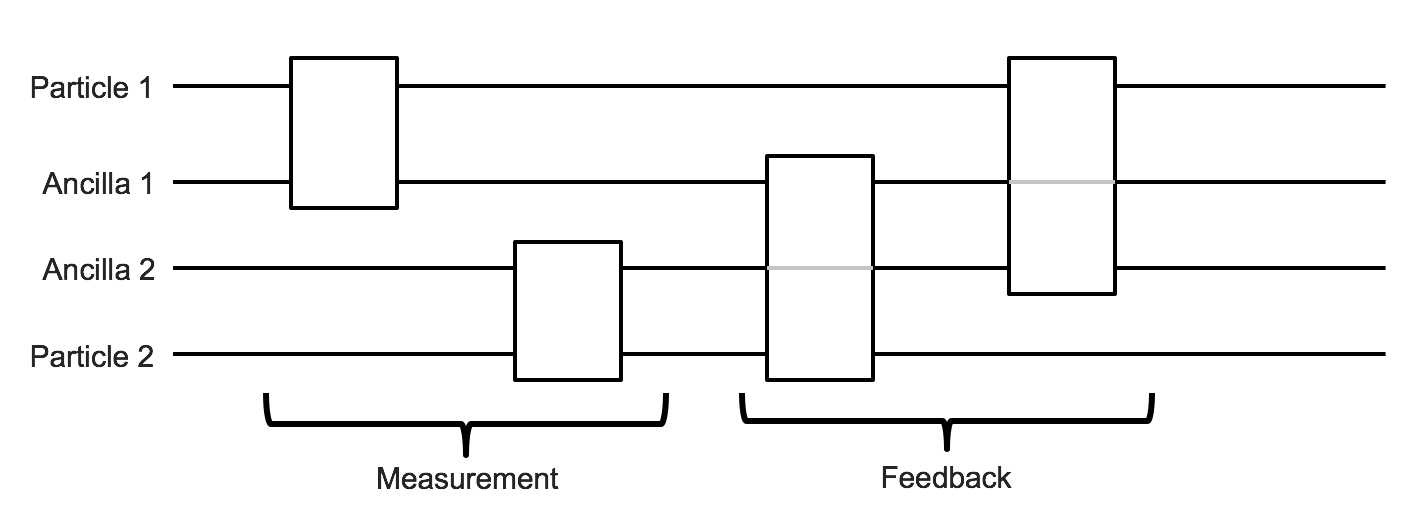
\includegraphics[width=0.8\textwidth]{Pairwise.png} 
\caption{Quantum circuit diagram illustrating the measurement-feedback mechanism by which ancillae propagate gravity.}
\label{measurement-feedback}
\end{figure*}

The KTM model can be divided into two cases: the pairwise case and the global case. In the pairwise case, a system requires two ancillae for each pair of gravitationally interacting particles. A system of two particles has only a single pair, thus two ancillae are required. A system with three particles has three pairs, thus six ancillae are required. The number of required ancillae increases rapidly as the number of particles increases. In the global case, only one ancilla is required for each particle in the system. Since the number of ancillae is at all times equal to number of particles in the global case, far fewer ancillae are required in the global case for systems containing a large number of particles. Interestingly, both cases require the same number of ancillae for $2$-particle systems. The two cases differ in the number of measurements per particle as well. To illustrate this, consider an $N$-particle system. In the pairwise case, each particle undergoes $N-1$ measurements, and the results of each measurement is used to give feedback to one of the other $N-1$ particles. In the global case, each particle undergoes only one measurement, and the results of this single measurement is used to give feedback to all of the other $N-1$ particles \cite{P7}.

%%%%%%%%%%%%%%%%%%%%%%%%%%%%%%%%%%%%%%%%%%%%%%%%%%%%%

\section{Testing the KTM Model}

To test the validity of the KTM model, the model's maximum theoretical visibilities estimates must be obtained and compared to results of an atomic fountain interference experiment, like those done by Kovachy et al. ~\cite{kovachy}. Visibility is a measure of the amount of a time a particle in a superposition can remain in a superposition, and it ranges from $0$ to $1$. A particle with a visibility of $1$ will maintain its superposition size for all time, and a particle with a visibility of $0$ collapses to a single state immediately. The atomic fountain experiments use large momentum transfer interferometers to put $^{87}$Rb atoms in a vertical spatial superposition. This is done using a sequence of $n$ $\frac{\pi}{2}$-pulses from a laser. The laser increases the superposition size for a total time $T$. The resulting superposition size of the atom is given by

\beq
\Delta x(t)=\frac{2\hbar n k  t}{m_a},
 \label{SP_size}
 \eeq
 
 for $t<T$ where $k$ is the laser's wave-number and $m_a$ is the mass of a $^{87}$Rb atom. The experiment found the visibility of the $^{87}$Rb atoms as a function of $n$.
 
Two estimates for the maximum theoretical visibility in both the pairwise and global case can be obtained. The maximum of the two estimates is the true maximum theoretical visibility, and each estimate is produced using it's own method: decoherence rate minimization (DRM) and heating rate minimization (HRM). Heating rate is equivalent to the rate at which energy is introduced to the system because of the ancillae. The DRM maximum theoretical visibility estimate for the pairwise case has been found to be inconsistent with experiment \cite{P3}. However, the HRM maximum visibility estimate for the pairwise case was later found to be greater than the previous estimate. For this reason, the HRM estimate is the pairwise case's true maximum theoretical visibility, and this visibility is consistent with values obtained through experiment, showing that it is possible for gravity to be a pairwise classical channel. Here, I obtain the DRM maximum visibility estimate for the global case. The HRM estimate for the global case has yet to be explored.

%%%%%%%%%%%%%%%%%%%%%%%%%%%%%%%%%%%%%%%%%%%%%%%%%%%%%

\section{DRM Maximum Visibility Estimate for the Global Case}

To derive the maximum visibility estimate through DRM, the global master equation must first be derived. The master equation describes how a gravitationally interacting system of particles changes in time under the KTM model. The master equation for the global case can be found easily from the already known pairwise master equation, given by

\beq
 \dot\rho_{pairwise} = -\frac{i}{\hbar}[\h H_0+\h V_0, \rho] 
 -\sum_{i} \sum_{j\neq i}\bigg(\frac{1}{4D_i}+\frac{K_{ij}^2D_j}{4\hbar^2}\bigg)[\h x_i, [\h x_i,\rho]],
 \label{ME_pairwise}
 \eeq

where $\h H_0 = \sum_{i}\frac{\h p_i^2}{2m_i}$ is the hamiltonian of the system in the absence of a gravitational field, and $\h V_0 = \sum_{i}\sum_{j\neq i} K_{ij}\h x_i \h x_j$ is an operator that accounts for gravity. The $i^{th}$ particle's momentum operator is represented by $\h p_i$, and its position operator is represented by $\h x_i$. The strength of the measurement and feedback interactions are gauged by the measurement strength $D_i$ and feedback strength $K_{ij} = 2\frac{Gm_{i}m_{j}}{d_{ij}^3}$ respectively, where $d_{ij}$ is the distance between particles $i$ and $j$ \cite{P3}. In eq.~\eqref{ME_pairwise}, the $\nicefrac{1}{4D_i}$ terms are the measurement terms and the $\nicefrac{K_{ij}^2D_j}{4\hbar^2}$ terms are the feedback terms. These terms account for the particles' measurement and feedback interactions with the ancillae. Note, the measurement terms depend only on the measurement strength of particle $i$, whereas the feedback terms depend on both the feedback strength between particles $i$ and $j$, and the measurement strength of particle $j$ because feedback depends on the result of the earlier measurement.
In the pairwise case, each particle undergoes $N-1$ measurements and $N-1$ feedbacks, which comes up in the master equation in the form of $N-1$ measurement and feedback terms produced by the $j\neq i$ sum. In the global case, the are still just as many feedbacks, but there is only a single measurement for each particle. This means that for the global case, the $j \neq i$ sum only applies to the feedback terms,

\beq
 \dot\rho_{global} = -\frac{i}{\hbar}[\h H_0+\h V_0, \rho] 
 -\sum_{i} \bigg(\frac{1}{4D_i}+\sum_{j\neq i}\frac{K_{ij}^2D_j}{4\hbar^2}\bigg)[\h x_i, [\h x_i,\rho]].
  \label{ME_global}
 \eeq

To compare the KTM model to the atomic fountain experiment, I approximate the experiment as a $2$-particle systems where one particle is a $^{87}$Rb atom and the other particle is the earth. In this case, the global master equation takes the form

\beq
 \dot\rho_{global} = -\frac{i}{\hbar}[\h H_0+\h V_0, \rho] 
 -\bigg(\frac{1}{4D_a}+\frac{K_{a\oplus}^2D_\oplus}{4\hbar^2}\bigg)[\h x_a, [\h x_a,\rho]]
  -\bigg(\frac{1}{4D_\oplus}+\frac{K_{a\oplus}^2D_a}{4\hbar^2}\bigg)[\h x_\oplus, [\h x_\oplus,\rho]].
  \label{ME_global_N1}
 \eeq
 
 The total decoherence rate of the system is defined to be the negative sum of the double commutators' coefficients multiplied by two factors of $\Delta x(t)$,
 
 \beq
\Gamma_{sys}=\bigg(\frac{1}{4D_a}+\frac{K_{a\oplus}^2D_\oplus}{4\hbar^2} + \frac{1}{4D_\oplus}+\frac{K_{a\oplus}^2D_a}{4\hbar^2}\bigg)\Delta x(t)^2.
\eeq

Using basic calculus, the values of $D_a$ and $D_\oplus$ that minimize $\Gamma_{sys}$ are found to be

\beq
D_a^{min} = D_\oplus^{min} = \frac{\hbar}{K_{a\oplus}}.
\label{D_min_N1}
 \eeq

Using eq.~\eqref{D_min_N1}, the minimum decoherence rate of the atom can then be expressed as

 \beq
\Gamma_a^{min}=\bigg(\frac{1}{4D_a^{min}}+\frac{K_{a\oplus}^2D_\oplus^{min}}{4\hbar^2}\bigg)\Delta x^2=\frac{K_{a\oplus} \Delta x^2}{2\hbar}.
\eeq
 
 From this, the maximum visibility estimate is found to be
 
\beq
V^{max}=\exp{\bigg(-2\int_0^T \Gamma_a^{min} dt\bigg)}=\exp{\bigg(\frac{-8n^2\hbar^2k^2T^3}{3m_a^2}\Gamma_a^{min}\bigg)} = \exp{\bigg(\frac{-8G\hbar M_\oplus n^2 k^2 T^3}{2 m_a R_\oplus^3}\bigg)}.
\label{Vis_N1}
\eeq

From eq.~\eqref{Vis_N1}, the model can be compared to the results of the atomic fountain experiment, however, approximating the earth as a point particle may not be a good approximation. Altamirano et al. found that approximating the earth as sphere composed of smaller bodies instead increases the visibility estimates considerably. For this reason, it is important to see the behaviour of visibility over large $N$ in the global case as well, where $N$ is the number of bodies the earth is composed of. Each of the $N$ bodies has mass $\nicefrac{M_\oplus}{N}$. Since each the N bodies has the same mass, they are assumed to have the same measurement strength $D_\oplus$. The atom is not assumed to have the same mass as  the earth-particles, so its measurement strength is still represented by $D_a$. The visibility equation above is for the $N=1$ case only. I have gone through the $N=2$ and $N=3$ cases by hand as well, and in doing so, the following can be shown:

 \beq
D_a^{min} = \frac{\hbar}{\sqrt{\sum_{i \neq a}K_{ia}^2}},
 \eeq
 
 \beq
D_\oplus^{min} = \hbar \sqrt{\frac{N}{\sum_{i\neq a}\sum_{j\neq i}K_{ij}^2 + \sum_{i \neq a}K_{ia}^2}},
 \eeq
and
\beq
\Gamma_a^{min} = \frac{1}{4D_a^{min}} + \frac{D_\oplus^{min}}{4\hbar^2}\sum_{i \neq a}K_{ia}^2.
\eeq

There are now two sums that must be solved in order to plot visibility: $\sum_{i \neq a}K_{ia}^2$ and $\sum_{i\neq a}\sum_{j\neq i}K_{ij}^2$. These are sums over the atom-earth and earth-earth feedbacks squared, respectively. These sums can be rewritten in an alternate form:

 \beq
\sum_{i \neq a}K_{ia}^2 = \bigg(\frac{2GM_\oplus m_a}{N}\bigg)^2 \sum_{i \neq a}d_{ia}^{-6},
\eeq
and 
 \beq
\sum_{i\neq a}\sum_{j\neq i}K_{ij}^2 = \bigg(\frac{2GM_\oplus^2}{N^2}\bigg)^2 \sum_{i\neq a}\sum_{j\neq i}d_{ij}^{-6}.
 \eeq
 
 It was decided to solve these distance sums numerically using a Python program. Given a lattice spacing, the program generates a cubic lattice with side lengths greater than the radius of the earth and with the centre lattice point centred at the origin. The x, y, and z co-ordinates of the lattice points, meant to represent earth-particles, are stored in arrays. The co-ordinates of all lattice points outside of the radius of the earth are set to NaN. The atom's co-ordinates are all set to $\nicefrac{R_\oplus}{\sqrt{3}}+2 \text{km}$. This places the atom just above the surface of the earth, instead being nearly directly on the surface like the atom in the atomic fountain experiments, in order to reduce noise for small $N$ since the results are very sensitive to the distance to the atom's nearest earth-particles. With the atom's and earth-particles' co-ordinates known, the distance sums become trivial so long as the program's time efficiency is not of great concern, thus a visibility plot can finally be obtained.
 
\begin{figure*}[ht!]
 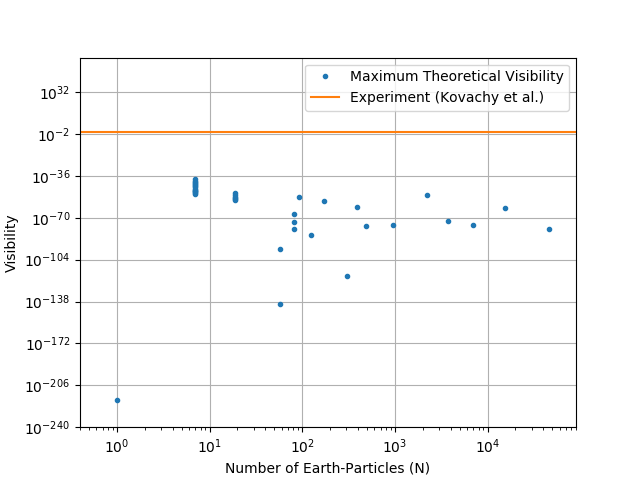
\includegraphics[width=.75\textwidth]{Vis.png} \caption{Comparing the DRM maximum theoretical visibility estimates to a value measured in the atomic fountain interference experiment. Here $M_\oplus  = 6 \times 10^{24}$ kg, $R_\oplus 6\times 10^3$ km, $\frac{\hbar k}{m_a} = 5.8 $ mm/s, $m_a = 1.4\times10^{-25}$ kg, and $T = 1.04$ s, and $n = 45$ \cite{kovachy}.}
\label{Vis}
\end{figure*}

 Fig.~\ref{Vis} shows the maximum theoretical visibility estimates produced using this numerical method, varying the number of earth-particles from $1$ to $45,817$. The value measured by the atomic fountain experiment is shown as well. The experimental visibility is constant at $0.28$ because the experiment was done with a virtually constant number of earth particles ($\sim 10^{50}$ \cite{site}). We seek to determine how many earth-particles must be used to approximate the earth in order for the maximum theoretical visibility to be greater than values from experiment. From fig.~\ref{Vis}, this appears to never occur. Though there is a sharp increase after the first point at $N=1$, the general trend of the points visually seems to either be constant or decreasing, but certainly not increasing. This means the maximum theoretical value will never be greater than the value from experiment. The DRM method does not yield visibility values compatible with experiment, though the HRM method must best done in order to definitively determine whether gravity could be a global local classical channel.

There are many other notable features in fig.~\ref{Vis}. Firstly, the outlier at $N=1$ is caused by the total earth-earth feedback being zero in this case only. Also, there are sometimes multiple points for a single value of $N$, for small $N$. This is because sometimes the number of lattice points that can fit within the earth does not change after the lattice spacing is decreased to calculate the maximum visibility at a new lattice spacing. The theoretical results are very noisy as well. This is due to the theoretical results being very sensitivity to the distance to earth-particles near the atom. Increasing N can introduce new lattice points very near the atom, and the introduction of these points has the a great effect on visibility for small $N$.

%%%%%%%%%%%%%%%%%%%%%%%%%%%%%%%%%%%%%%%%%%%%%%%%%%%%%

\pagebreak[4]
\section{Conclusion}
To test the KTM model's validity completely, four maximum visibility estimates are required. Two estimates from both the pairwise and global case: one estimate using DRM and one estimate using HRM. Altamirano et al. and Breault obtained both the DRM and HRM estimates for the pairwise case \cite{P3, breault}, and the DRM estimate for the global case is obtained here. A process similar to that used by Altamirano et al. to derive the DRM pairwise estimate is used here, though the numerical evaluation of the sums is unique to the global case.

It has been shown that the maximum visibility estimates produced by minimizing decoherence rate are far too small to be consistent with the atomic fountain experiment. The visibility does not visually appear to be increasing with the number of earth-particles used to model the earth, though this can't not be stated with a high degree of certainty due to the amount of noise present in fig.~\ref{Vis}. It is expected for the noise due to sensitivity to earth-particle distance to decrease with $N$ since small changes in the number of lattice points does not greatly change the local distribution of points near the atom for large $N$. This problem can be solved by running the program for smaller lattice spacings to determine the visibility's large N behaviour, though the program used to produce fig.~\ref{Vis} runs very slow for $N>10000$. More time efficient numerical methods should be explored, specifically regarding the earth-earth distance sum. Preforming this sum is the slowest step of the program by far for large $N$, it currently takes approximately $N$ times longer to preform than the atom-earth distance sum.

The next logical step to take regarding this research is to obtain the HRM maximum theoretical visibility estimate for the global case. This is required to determine whether the DRM estimate or the HRM estimate is the true maximum theoretical visibility for the global case. Until the global HRM estimate is known, it is impossible to know whether gravity could be a global local classical channel. Obtaining the global HRM estimate is not expected to be of great difficulty since the global master equation is now known and a process similar to the one used in the pairwise case by Breault can be followed \cite{breault}.

%%%%%%%%%%%%%%%%%%%%%%%%%%%%%%%%%%%%%%%%%%%%%%%%%%%%%%

\pagebreak[4]
\section{Acknowledgments}
I would like to thank my supervisor, Professor Robert Mann, and Natacha Altamirano for the guidance and direction they offered throughout the course of this project. Completing so much within the time constraints of the project would have been impossible without their assistance.

%%%%%%%%%%%%%%%%%%%%%%%%%%%%%%%%%%%%%%%%%%%%%%%%%%%%%%
\begingroup\raggedright\begin{thebibliography}{10}

%\section{References}

\bibitem{PI}
Quantum Gravity. (n.d.). Retrieved from https://www.perimeterinstitute.ca/research/research-areas/quantum-gravity.

\bibitem{no_QG_evidence}
D.~N. Page and C.~D. Geilker, ``{Indirect Evidence for Quantum Gravity},''
\href{http://dx.doi.org/10.1103/PhysRevLett.47.979}{{\em Phys. Rev. Lett.}
  {\bfseries 47}, 979--982 (1981)}.
%%CITATION = PRLTA,47,979;%%.

\bibitem{KTM1}
D.~{Kafri} and J.~M. {Taylor}, ``{A noise inequality for classical forces},''
  {\em ArXiv e-prints} (2013), \href{http://arxiv.org/abs/1311.4558}{{\ttfamily
  arXiv:1311.4558 [quant-ph]}}.

\bibitem{KTM2}
D.~Kafri, J.~M. Taylor, and G.~J. Milburn, ``{A classical channel model for
  gravitational decoherence},''
  \href{http://dx.doi.org/10.1088/1367-2630/16/6/065020}{{\em New J. Phys.}
  {\bfseries 16}, 065020 (2014)},
\href{http://arxiv.org/abs/1401.0946}{{\ttfamily arXiv:1401.0946 [quant-ph]}}.
%%CITATION = ARXIV:1401.0946;%%.

\bibitem{KTM3}
D.~Kafri, G.~J. Milburn, and J.~M. Taylor, ``{Bounds on quantum communication
  via Newtonian gravity},''
\href{http://dx.doi.org/10.1088/1367-2630/17/1/015006}{{\em New J. Phys.}
  {\bfseries 17}, 015006 (2015)}.
%%CITATION = NJOPF,17,015006;%%.

\bibitem{P6}
N.~Altamirano, P.~Corona-Ugalde, K.~E. Khosla, R.~B. Mann, and M.~Zych, ``{Emergent dark energy via decoherence in quantum
interactions},''{(2017)}
   \href{https://arxiv.org/pdf/1605.05980.pdf},
{{\ttfamily arXiv:1605.05980v2 [gr-qc]}}.
%%CITATION = ARXIV:1605.04312;%%.

\bibitem{P2}
N.~Altamirano, P.~Corona-Ugalde, R.~B. Mann, and M.~Zych, ``{Unitarity,
  Feedback, Interactions -- Dynamics Emergent from Repeated Measurements},''
   \href{http://iopscience.iop.org/article/10.1088/1367-2630/aa551b}{{\em New Journal of Physics}
 (2016)},
\href{http://arxiv.org/abs/1605.04312}{{\ttfamily arXiv:1605.04312
  [quant-ph]}}.
%%CITATION = ARXIV:1605.04312;%%.

\bibitem{P3}
N.~Altamirano, P.~Corona-Ugalde, R.~B. Mann, and M.~Zych, ``{Gravity is not a Pairwise Classical Channel},''
   {(2016)},
\href{http://arxiv.org/abs/1612.07735v1}{{\ttfamily arXiv:1612.07735v1
  [quant-ph]}}.
%%CITATION = ARXIV:1605.04312;%%.

\bibitem{kovachy}
T.~Kovachy, P.~Asenbaum, C.~Overstreet, C.~Donnelly, S.~Dickerson,
  A.~Sugarbaker, J.~Hogan, and M.~Kasevich, ``Quantum superposition at the
  half-metre scale,'' {\em Nature} {\bfseries 528}, 530--533 (2015).

\bibitem{breault}
Breault, J. G. (2018). Gravity May be a Local Classical Channel.

\bibitem{P7}
Khosla, K., Altamirano, N. (2016). Detecting gravitational decoherence with clocks: Limits on temporal resolution from a classical channel model of gravity.

\bibitem{site}
Inquiring Minds. Retrieved April 13, 2018, from http://www.fnal.gov/pub/science/inquiring/questions/atoms.html

\end{thebibliography}\endgroup

\end{document}






















